% !TEX TS-program = pdflatex
% !TEX encoding = UTF-8 Unicode

% This is a simple template for a LaTeX document using the "article" class.
% See "book", "report", "letter" for other types of document.

\documentclass[11pt]{article} % use larger type; default would be 10pt

\usepackage[utf8]{inputenc} % set input encoding (not needed with XeLaTeX)


%%% PAGE DIMENSIONS
\usepackage{geometry} % to change the page dimensions
\geometry{a4paper} % or letterpaper (US) or a5paper or....


\usepackage{graphicx} % support the \includegraphics command and options

% \usepackage[parfill]{parskip} % Activate to begin paragraphs with an empty line rather than an indent

%%% PACKAGES
\usepackage{booktabs} % for much better looking tables
\usepackage{array} % for better arrays (eg matrices) in maths
\usepackage{paralist} % very flexible & customisable lists (eg. enumerate/itemize, etc.)
\usepackage{verbatim} % adds environment for commenting out blocks of text & for better verbatim
\usepackage{subfig} % make it possible to include more than one captioned figure/table in a single float
\usepackage{cite}
% These packages are all incorporated in the memoir class to one degree or another...

%%% HEADERS & FOOTERS
\usepackage{fancyhdr} % This should be set AFTER setting up the page geometry
\pagestyle{fancy} % options: empty , plain , fancy
\renewcommand{\headrulewidth}{0pt} % customise the layout...
\lhead{}\chead{}\rhead{}
\lfoot{}\cfoot{\thepage}\rfoot{}

%%% SECTION TITLE APPEARANCE
\usepackage{sectsty}
\allsectionsfont{\sffamily\mdseries\upshape} % (See the fntguide.pdf for font help)
% (This matches ConTeXt defaults)

%%% ToC (table of contents) APPEARANCE
\usepackage[nottoc,notlof,notlot]{tocbibind} % Put the bibliography in the ToC
\usepackage[titles,subfigure]{tocloft} % Alter the style of the Table of Contents
\graphicspath{ {Images/} }
\renewcommand{\cftsecfont}{\rmfamily\mdseries\upshape}
\renewcommand{\cftsecpagefont}{\rmfamily\mdseries\upshape} % No bold!



\title{Mapping the Brain: An Introduction to Connectomics\\Creating Classifiers for the Identification of Gender in Brain Graph Data}
\author{Chris Micek, Addison Wright, Monica Rodriguez-Fernandez}
%\date{} % Activate to display a given date or no date (if empty),
         % otherwise the current date is printed 

\begin{document}
\maketitle

\section{Abstract}

An abundance of MR brain graph data has recently been acquired via the m2g pipeline, which associate subjects with covariates such as age and gender. We focus specifically on the Southwest China Data set. However, these data have yet to be analyzed; moreover, feature importance in graph classification is not well established. Here we present an ensemble of MATLAB classifiers implemented to classify MR brain graph data from the Desikan atlas based on gender, as well as features deemed important by our linear classifier. We see that simply vectorizing the graphs and treating each one as a high dimensional point proves to be a powerful method when trying to classify gender. Possible future work may entail optimizing each classifier, attempting to classify based on non-binary covariates, extrapolating this methodology to other atlases and experimenting with other feature selections given a particular graph.

\section{Results}

After analysis the following was very clear: 
Weighted Graphs allow for increased classification rates;
Treating the graphs as "full" matrices vs. "sparse" matrices considerably improves classification rates in MATLAB; 
Certain classifiers perform better given Binary or Weighted graphs. 
Binary Ranks:
SVM,
Voting,
KNN,
Trees,
Linear,
Adaboost
Weighted:
Trees and Adaboost (tie),
Voting,
Linear,
KNN,
SVM.
\newpage
\section{Figures}
\subsection{Binary}

\begin{figure}[!htb]
	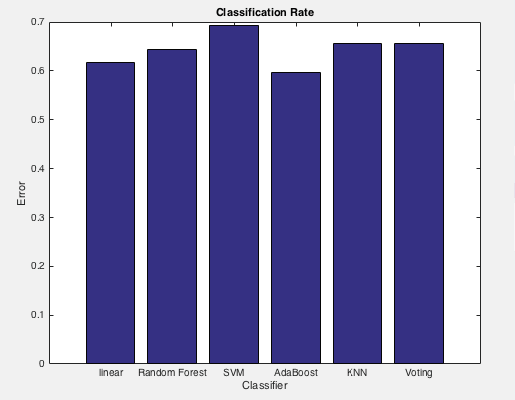
\includegraphics{BinBar}
	\caption{Classification rate for binary data.}
\end{figure}
\begin{figure}
	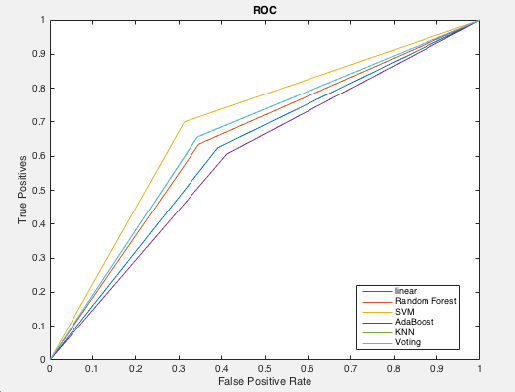
\includegraphics{BinROC}
	\caption{ROC curve for binary data.}
\end{figure}
\newpage
\subsection{Weighted}
\begin{figure}[!htb]
	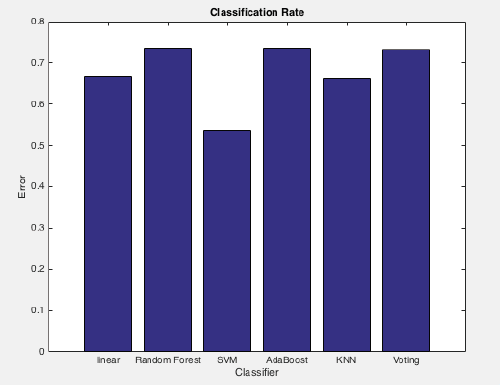
\includegraphics{WBar}
	\caption{Classification rate for weighted data.}
\end{figure}
\begin{figure}
	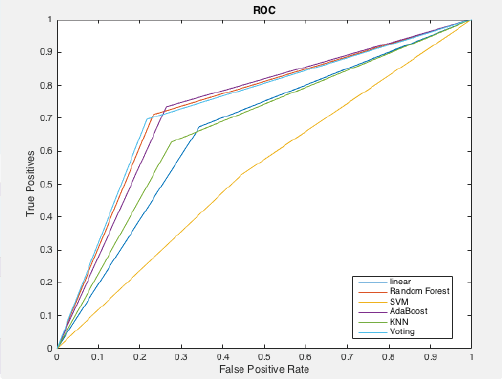
\includegraphics{WROC}
	\caption{ROC curve for weighted data.}
\end{figure}

\end{document}
